% Options for packages loaded elsewhere
\PassOptionsToPackage{unicode}{hyperref}
\PassOptionsToPackage{hyphens}{url}
%
\documentclass[
]{article}
\usepackage{lmodern}
\usepackage{amssymb,amsmath}
\usepackage{ifxetex,ifluatex}
\ifnum 0\ifxetex 1\fi\ifluatex 1\fi=0 % if pdftex
  \usepackage[T1]{fontenc}
  \usepackage[utf8]{inputenc}
  \usepackage{textcomp} % provide euro and other symbols
\else % if luatex or xetex
  \usepackage{unicode-math}
  \defaultfontfeatures{Scale=MatchLowercase}
  \defaultfontfeatures[\rmfamily]{Ligatures=TeX,Scale=1}
\fi
% Use upquote if available, for straight quotes in verbatim environments
\IfFileExists{upquote.sty}{\usepackage{upquote}}{}
\IfFileExists{microtype.sty}{% use microtype if available
  \usepackage[]{microtype}
  \UseMicrotypeSet[protrusion]{basicmath} % disable protrusion for tt fonts
}{}
\makeatletter
\@ifundefined{KOMAClassName}{% if non-KOMA class
  \IfFileExists{parskip.sty}{%
    \usepackage{parskip}
  }{% else
    \setlength{\parindent}{0pt}
    \setlength{\parskip}{6pt plus 2pt minus 1pt}}
}{% if KOMA class
  \KOMAoptions{parskip=half}}
\makeatother
\usepackage{xcolor}
\IfFileExists{xurl.sty}{\usepackage{xurl}}{} % add URL line breaks if available
\IfFileExists{bookmark.sty}{\usepackage{bookmark}}{\usepackage{hyperref}}
\hypersetup{
  pdftitle={STAT 428: Homework 3:   Chapter 3 and Chapters 5 Monte Carlo Methods},
  pdfauthor={Du, Yuting, yutingd3   Collaborated with: Sun, Yifan, yifans8},
  hidelinks,
  pdfcreator={LaTeX via pandoc}}
\urlstyle{same} % disable monospaced font for URLs
\usepackage[margin=1in]{geometry}
\usepackage{color}
\usepackage{fancyvrb}
\newcommand{\VerbBar}{|}
\newcommand{\VERB}{\Verb[commandchars=\\\{\}]}
\DefineVerbatimEnvironment{Highlighting}{Verbatim}{commandchars=\\\{\}}
% Add ',fontsize=\small' for more characters per line
\usepackage{framed}
\definecolor{shadecolor}{RGB}{248,248,248}
\newenvironment{Shaded}{\begin{snugshade}}{\end{snugshade}}
\newcommand{\AlertTok}[1]{\textcolor[rgb]{0.94,0.16,0.16}{#1}}
\newcommand{\AnnotationTok}[1]{\textcolor[rgb]{0.56,0.35,0.01}{\textbf{\textit{#1}}}}
\newcommand{\AttributeTok}[1]{\textcolor[rgb]{0.77,0.63,0.00}{#1}}
\newcommand{\BaseNTok}[1]{\textcolor[rgb]{0.00,0.00,0.81}{#1}}
\newcommand{\BuiltInTok}[1]{#1}
\newcommand{\CharTok}[1]{\textcolor[rgb]{0.31,0.60,0.02}{#1}}
\newcommand{\CommentTok}[1]{\textcolor[rgb]{0.56,0.35,0.01}{\textit{#1}}}
\newcommand{\CommentVarTok}[1]{\textcolor[rgb]{0.56,0.35,0.01}{\textbf{\textit{#1}}}}
\newcommand{\ConstantTok}[1]{\textcolor[rgb]{0.00,0.00,0.00}{#1}}
\newcommand{\ControlFlowTok}[1]{\textcolor[rgb]{0.13,0.29,0.53}{\textbf{#1}}}
\newcommand{\DataTypeTok}[1]{\textcolor[rgb]{0.13,0.29,0.53}{#1}}
\newcommand{\DecValTok}[1]{\textcolor[rgb]{0.00,0.00,0.81}{#1}}
\newcommand{\DocumentationTok}[1]{\textcolor[rgb]{0.56,0.35,0.01}{\textbf{\textit{#1}}}}
\newcommand{\ErrorTok}[1]{\textcolor[rgb]{0.64,0.00,0.00}{\textbf{#1}}}
\newcommand{\ExtensionTok}[1]{#1}
\newcommand{\FloatTok}[1]{\textcolor[rgb]{0.00,0.00,0.81}{#1}}
\newcommand{\FunctionTok}[1]{\textcolor[rgb]{0.00,0.00,0.00}{#1}}
\newcommand{\ImportTok}[1]{#1}
\newcommand{\InformationTok}[1]{\textcolor[rgb]{0.56,0.35,0.01}{\textbf{\textit{#1}}}}
\newcommand{\KeywordTok}[1]{\textcolor[rgb]{0.13,0.29,0.53}{\textbf{#1}}}
\newcommand{\NormalTok}[1]{#1}
\newcommand{\OperatorTok}[1]{\textcolor[rgb]{0.81,0.36,0.00}{\textbf{#1}}}
\newcommand{\OtherTok}[1]{\textcolor[rgb]{0.56,0.35,0.01}{#1}}
\newcommand{\PreprocessorTok}[1]{\textcolor[rgb]{0.56,0.35,0.01}{\textit{#1}}}
\newcommand{\RegionMarkerTok}[1]{#1}
\newcommand{\SpecialCharTok}[1]{\textcolor[rgb]{0.00,0.00,0.00}{#1}}
\newcommand{\SpecialStringTok}[1]{\textcolor[rgb]{0.31,0.60,0.02}{#1}}
\newcommand{\StringTok}[1]{\textcolor[rgb]{0.31,0.60,0.02}{#1}}
\newcommand{\VariableTok}[1]{\textcolor[rgb]{0.00,0.00,0.00}{#1}}
\newcommand{\VerbatimStringTok}[1]{\textcolor[rgb]{0.31,0.60,0.02}{#1}}
\newcommand{\WarningTok}[1]{\textcolor[rgb]{0.56,0.35,0.01}{\textbf{\textit{#1}}}}
\usepackage{graphicx,grffile}
\makeatletter
\def\maxwidth{\ifdim\Gin@nat@width>\linewidth\linewidth\else\Gin@nat@width\fi}
\def\maxheight{\ifdim\Gin@nat@height>\textheight\textheight\else\Gin@nat@height\fi}
\makeatother
% Scale images if necessary, so that they will not overflow the page
% margins by default, and it is still possible to overwrite the defaults
% using explicit options in \includegraphics[width, height, ...]{}
\setkeys{Gin}{width=\maxwidth,height=\maxheight,keepaspectratio}
% Set default figure placement to htbp
\makeatletter
\def\fps@figure{htbp}
\makeatother
\setlength{\emergencystretch}{3em} % prevent overfull lines
\providecommand{\tightlist}{%
  \setlength{\itemsep}{0pt}\setlength{\parskip}{0pt}}
\setcounter{secnumdepth}{-\maxdimen} % remove section numbering
% https://github.com/rstudio/rmarkdown/issues/337
\let\rmarkdownfootnote\footnote%
\def\footnote{\protect\rmarkdownfootnote}

% https://github.com/rstudio/rmarkdown/pull/252
\usepackage{titling}
\setlength{\droptitle}{-2em}

\pretitle{\vspace{\droptitle}\centering\huge}
\posttitle{\par}

\preauthor{\centering\large\emph}
\postauthor{\par}

\predate{\centering\large\emph}
\postdate{\par}

\title{STAT 428: Homework 3: Chapter 3 and Chapters 5 Monte Carlo Methods}
\author{Du, Yuting, yutingd3 Collaborated with: Sun, Yifan, yifans8}
\date{}

\begin{document}
\maketitle

{
\setcounter{tocdepth}{2}
\tableofcontents
}
\begin{center}\rule{0.5\linewidth}{\linethickness}\end{center}

Please refer to the {[}\textbf{detailed homework policy document}{]} on
Course Page for information about homework formatting, submission, and
grading.

\begin{center}\rule{0.5\linewidth}{\linethickness}\end{center}

\hypertarget{exercise-1}{%
\subsection{Exercise 1}\label{exercise-1}}

\textbf{Sampling discrete distributions.}

\textbf{(a)} Design an algorithm to simulate from a
\texttt{Geometric(p)} (where \(x\) is the number of failures until the
first success) distribution via the inverse transform method.
\emph{(Hint: Recall that Geometric random variables are just the number
of Bernoulli random variables with the same parameter \texttt{p} until
you get a success. So just focus on simulating \texttt{n} Bernoulli
variables and then you can transform to Geometric ones.)}

\textbf{(b)} Write R code to generate a sample following the Geometric
distribution based on your designed algorithm in the previous part. Use
\(n=1000\) sample size and \(p=0.4\). Then, estimate the expected value
of this Geometric distribution via Monte Carlo integration to check if
your estimates match the theoretically expected value of Geometric
distribution or not.

\hypertarget{solution-1}{%
\subsection{Solution 1}\label{solution-1}}

\textbf{(a)} Design an algorithm to simulate from a
\texttt{Geometric(p)} (where \(x\) is the number of failures until the
first success) distribution via the inverse transform method.
\emph{(Hint: Recall that Geometric random variables are just the number
of Bernoulli random variables with the same parameter \texttt{p} until
you get a success. So just focus on simulating \texttt{n} Bernoulli
variables and then you can transform to Geometric ones.)} generare a
Bernoulli(p) rv, then the sicrete inverse-transformation method yields:
1. Generate U\textasciitilde unif(0,1) 2. Set X = 0 if U \textless= 1-p;
X = 1 if U \textgreater{} 1-p Then repeat this process n times and
record the first x hitting 1

\textbf{(b)} Write R code to generate a sample following the Geometric
distribution based on your designed algorithm in the previous part. Use
\(n=1000\) sample size and \(p=0.4\). Then, estimate the expected value
of this Geometric distribution via Monte Carlo integration to check if
your estimates match the theoretically expected value of Geometric
distribution or not.

\begin{Shaded}
\begin{Highlighting}[]
\NormalTok{u =}\StringTok{ }\KeywordTok{numeric}\NormalTok{()}
\NormalTok{k =}\StringTok{ }\KeywordTok{numeric}\NormalTok{()}

\NormalTok{geo =}\StringTok{ }\ControlFlowTok{function}\NormalTok{(n,p)\{}
\ControlFlowTok{for}\NormalTok{ (i }\ControlFlowTok{in} \DecValTok{1}\OperatorTok{:}\NormalTok{n) \{}
\NormalTok{  u[i] =}\StringTok{ }\KeywordTok{runif}\NormalTok{(}\DecValTok{1}\NormalTok{)}
  \ControlFlowTok{if}\NormalTok{ (u[i] }\OperatorTok{<}\StringTok{ }\NormalTok{p)}
\NormalTok{    k[i] =}\StringTok{ }\DecValTok{0}
  \ControlFlowTok{else}
\NormalTok{    k[i] =}\StringTok{ }\KeywordTok{ceiling}\NormalTok{(}\KeywordTok{log}\NormalTok{(}\DecValTok{1}\OperatorTok{-}\NormalTok{u[i])}\OperatorTok{/}\KeywordTok{log}\NormalTok{(}\DecValTok{1}\OperatorTok{-}\NormalTok{p))}\OperatorTok{-}\DecValTok{1}\CommentTok{#inverse cdf}
\NormalTok{\}}
  \KeywordTok{return}\NormalTok{(k)}
\NormalTok{\}}

\KeywordTok{mean}\NormalTok{(}\KeywordTok{geo}\NormalTok{(}\DecValTok{1000}\NormalTok{, }\FloatTok{0.4}\NormalTok{))}
\end{Highlighting}
\end{Shaded}

\begin{verbatim}
## [1] 1.513
\end{verbatim}

\begin{Shaded}
\begin{Highlighting}[]
\KeywordTok{mean}\NormalTok{(}\KeywordTok{rgeom}\NormalTok{(}\DecValTok{1000}\NormalTok{,}\FloatTok{0.4}\NormalTok{))}
\end{Highlighting}
\end{Shaded}

\begin{verbatim}
## [1] 1.548
\end{verbatim}

\hypertarget{exercise-2}{%
\subsection{Exercise 2}\label{exercise-2}}

\textbf{Monte Carlo Integration.} Use Monte Carlo integration to
estimate

\textbf{(a)} \[\int_{0}^{2} \cos(x*e^x) dx\] \textbf{(b)}
\[\int_{0}^{1}\int_{0}^{1} e^{-(x+y)^2}(x^2+y) dx dy\] \textbf{(c)}
\[\int_{0}^{4}\int_{0}^{3} e^{-(x+y)^2}(x^2+y) dx dy\]

\hypertarget{solution-2}{%
\subsection{Solution 2}\label{solution-2}}

\textbf{(a)} \[\int_{0}^{2} \cos(x*e^x) dx\]

\begin{Shaded}
\begin{Highlighting}[]
\NormalTok{u1 <-}\StringTok{ }\KeywordTok{runif}\NormalTok{(}\DecValTok{1000}\NormalTok{, }\DecValTok{0}\NormalTok{, }\DecValTok{2}\NormalTok{)}
\NormalTok{x1 <-}\StringTok{ }\DecValTok{2}\OperatorTok{*}\KeywordTok{mean}\NormalTok{(}\KeywordTok{cos}\NormalTok{(}\KeywordTok{exp}\NormalTok{(u1)}\OperatorTok{*}\NormalTok{u1))}
\NormalTok{x1}
\end{Highlighting}
\end{Shaded}

\begin{verbatim}
## [1] 0.3614
\end{verbatim}

\textbf{(b)} \[\int_{0}^{1}\int_{0}^{1} e^{-(x+y)^2}(x^2+y) dx dy\]

\begin{Shaded}
\begin{Highlighting}[]
\NormalTok{x <-}\StringTok{ }\KeywordTok{runif}\NormalTok{(}\DecValTok{1000}\NormalTok{)}
\NormalTok{y <-}\StringTok{ }\KeywordTok{runif}\NormalTok{(}\DecValTok{1000}\NormalTok{)}
\NormalTok{x2 <-}\StringTok{ }\KeywordTok{mean}\NormalTok{(}\KeywordTok{exp}\NormalTok{(}\OperatorTok{-}\NormalTok{(x}\OperatorTok{+}\NormalTok{y)}\OperatorTok{^}\DecValTok{2}\NormalTok{) }\OperatorTok{*}\StringTok{ }\NormalTok{(x}\OperatorTok{^}\DecValTok{2}\OperatorTok{+}\NormalTok{y))}
\NormalTok{x2}
\end{Highlighting}
\end{Shaded}

\begin{verbatim}
## [1] 0.2388
\end{verbatim}

\textbf{(c)} \[\int_{0}^{4}\int_{0}^{3} e^{-(x+y)^2}(x^2+y) dx dy\]

\begin{Shaded}
\begin{Highlighting}[]
\NormalTok{x <-}\StringTok{ }\KeywordTok{runif}\NormalTok{(}\DecValTok{1000}\NormalTok{, }\DecValTok{0}\NormalTok{, }\DecValTok{3}\NormalTok{)}
\NormalTok{y <-}\StringTok{ }\KeywordTok{runif}\NormalTok{(}\DecValTok{1000}\NormalTok{, }\DecValTok{0}\NormalTok{, }\DecValTok{4}\NormalTok{)}
\NormalTok{x3 <-}\StringTok{ }\DecValTok{12}\OperatorTok{*}\KeywordTok{mean}\NormalTok{(}\KeywordTok{exp}\NormalTok{(}\OperatorTok{-}\NormalTok{(x}\OperatorTok{+}\NormalTok{y)}\OperatorTok{^}\DecValTok{2}\NormalTok{) }\OperatorTok{*}\StringTok{ }\NormalTok{(x}\OperatorTok{^}\DecValTok{2}\OperatorTok{+}\NormalTok{y))}
\NormalTok{x3}
\end{Highlighting}
\end{Shaded}

\begin{verbatim}
## [1] 0.3983
\end{verbatim}

\hypertarget{exercise-3}{%
\subsection{Exercise 3}\label{exercise-3}}

\textbf{Variance reduction in Monte Carlo Integration: Antithetic
sampling.} Let us consider the simple integral
\[ \int_0^1 \log(x+1) \; dx. \] (where \(\log(x)=\ln(x)\))

\textbf{(a)} Use Monte Carlo integration with \(k = 1000\) iterations to
approximate this integral. Call this approximate value \(I_0\).

\textbf{(b)} Find the error of this approximation by repeating this
simulation \(n = 1000\) times and calculating standard error of this
estimator. Call this error \(E_0\). \emph{(Hint: Rememeber standard
error = standard deviation of the estimator from multiple simulations.)}

\textbf{(c)} Note that if \(U \sim Unif(0,1)\), then
\(1 - U \sim Unif(0,1)\) also. Obtain a Monte Carlo approximation of the
integral using \(k_1 = 500\) iterations and uniform distribution
\emph{(This step is same as part (a))}. Call this \(I_{11}\). Obtain
another MC approximation (call this \(I_{12}\)) using \(k_2 = 500\)
iterations and the antithetic uniform distribution \emph{(Which means in
part (a), now use 1-U instead of U.)} Find the average of these two
approximations and call it \(I_1 = (I_{11}+I_{12})/2\). What is \(I_1\)
an approximation of? Compare it to \(I_0\).

\textbf{(d)} Repeat step (c) 1000 times and find the standard error of
the estimator \(I_1\). Compare this error with the error \(E_0\) from
(b).

\hypertarget{solution-3}{%
\subsection{Solution 3}\label{solution-3}}

\textbf{(a)} Use Monte Carlo integration with \(k = 1000\) iterations to
approximate this integral. Call this approximate value \(I_0\).

\begin{Shaded}
\begin{Highlighting}[]
\KeywordTok{set.seed}\NormalTok{(}\DecValTok{123}\NormalTok{)}
\NormalTok{u =}\StringTok{ }\KeywordTok{runif}\NormalTok{(}\DecValTok{1000}\NormalTok{)}
\NormalTok{I0 =}\StringTok{ }\KeywordTok{mean}\NormalTok{(}\KeywordTok{log}\NormalTok{(u}\OperatorTok{+}\DecValTok{1}\NormalTok{))}
\NormalTok{I0}
\end{Highlighting}
\end{Shaded}

\begin{verbatim}
## [1] 0.3846
\end{verbatim}

\textbf{(b)} Find the error of this approximation by repeating this
simulation \(n = 1000\) times and calculating standard error of this
estimator. Call this error \(E_0\). \emph{(Hint: Rememeber standard
error = standard deviation of the estimator from multiple simulations.)}

\begin{Shaded}
\begin{Highlighting}[]
\KeywordTok{set.seed}\NormalTok{(}\DecValTok{123}\NormalTok{)}
\NormalTok{u =}\StringTok{ }\KeywordTok{runif}\NormalTok{(}\DecValTok{1000}\NormalTok{)}
\NormalTok{x =}\StringTok{ }\KeywordTok{numeric}\NormalTok{()}
\ControlFlowTok{for}\NormalTok{(i }\ControlFlowTok{in} \DecValTok{1}\OperatorTok{:}\StringTok{ }\DecValTok{1000}\NormalTok{)\{}
\NormalTok{  x[i] =}\StringTok{ }\KeywordTok{mean}\NormalTok{(}\KeywordTok{log}\NormalTok{(u[i]}\OperatorTok{+}\DecValTok{1}\NormalTok{))}
\NormalTok{\}}

\NormalTok{E0 <-}\StringTok{ }\KeywordTok{sd}\NormalTok{(x)}\OperatorTok{/}\KeywordTok{sqrt}\NormalTok{(}\DecValTok{1000}\NormalTok{)}
\NormalTok{E0}
\end{Highlighting}
\end{Shaded}

\begin{verbatim}
## [1] 0.006231
\end{verbatim}

\textbf{(c)} Note that if \(U \sim Unif(0,1)\), then
\(1 - U \sim Unif(0,1)\) also. Obtain a Monte Carlo approximation of the
integral using \(k_1 = 500\) iterations and uniform distribution
\emph{(This step is same as part (a))}. Call this \(I_{11}\). Obtain
another MC approximation (call this \(I_{12}\)) using \(k_2 = 500\)
iterations and the antithetic uniform distribution \emph{(Which means in
part (a), now use 1-U instead of U.)} Find the average of these two
approximations and call it \(I_1 = (I_{11}+I_{12})/2\). What is \(I_1\)
an approximation of? Compare it to \(I_0\).

\begin{Shaded}
\begin{Highlighting}[]
\KeywordTok{set.seed}\NormalTok{(}\DecValTok{123}\NormalTok{)}
\NormalTok{k1 <-}\StringTok{ }\DecValTok{500}
\NormalTok{u1 <-}\StringTok{ }\KeywordTok{runif}\NormalTok{(k1)}
\NormalTok{I11 <-}\StringTok{ }\KeywordTok{mean}\NormalTok{(}\KeywordTok{log}\NormalTok{(u1}\OperatorTok{+}\DecValTok{1}\NormalTok{))}

\KeywordTok{set.seed}\NormalTok{(}\DecValTok{124}\NormalTok{)}
\NormalTok{k2 <-}\StringTok{ }\DecValTok{500}
\NormalTok{u2 <-}\StringTok{ }\KeywordTok{runif}\NormalTok{(k2)}
\NormalTok{I12 <-}\StringTok{ }\KeywordTok{mean}\NormalTok{(}\KeywordTok{log}\NormalTok{(}\DecValTok{1}\OperatorTok{-}\NormalTok{u2 }\OperatorTok{+}\StringTok{ }\DecValTok{1}\NormalTok{))}

\NormalTok{I1 <-}\StringTok{ }\NormalTok{(I11 }\OperatorTok{+}\StringTok{ }\NormalTok{I12)}\OperatorTok{/}\DecValTok{2}
\NormalTok{I1}
\end{Highlighting}
\end{Shaded}

\begin{verbatim}
## [1] 0.3856
\end{verbatim}

I1 is similar to I0. I0 can be explained as the expectation of the
average of two results in Monte Carlo integration

\textbf{(d)} Repeat step (c) 1000 times and find the standard error of
the estimator \(I_1\). Compare this error with the error \(E_0\) from
(b).

\begin{Shaded}
\begin{Highlighting}[]
\NormalTok{I1 =}\StringTok{ }\KeywordTok{numeric}\NormalTok{()}
\NormalTok{I11 =}\StringTok{ }\KeywordTok{numeric}\NormalTok{()}
\NormalTok{I12 =}\StringTok{ }\KeywordTok{numeric}\NormalTok{()}


\ControlFlowTok{for}\NormalTok{(i }\ControlFlowTok{in} \DecValTok{1}\OperatorTok{:}\DecValTok{1000}\NormalTok{)\{}
\NormalTok{  k1 <-}\StringTok{ }\DecValTok{500}
\NormalTok{  u1 <-}\StringTok{ }\KeywordTok{runif}\NormalTok{(}\DecValTok{500}\NormalTok{)}
\NormalTok{  I11[i] <-}\StringTok{ }\KeywordTok{mean}\NormalTok{(}\KeywordTok{log}\NormalTok{(u1 }\OperatorTok{+}\StringTok{ }\DecValTok{1}\NormalTok{))}
  
\NormalTok{  k2 <-}\StringTok{ }\DecValTok{500}
\NormalTok{  u2 <-}\StringTok{ }\KeywordTok{runif}\NormalTok{(}\DecValTok{500}\NormalTok{)}
\NormalTok{  I12[i] <-}\StringTok{ }\KeywordTok{mean}\NormalTok{(}\KeywordTok{log}\NormalTok{(}\DecValTok{1}\OperatorTok{-}\NormalTok{u2}\OperatorTok{+}\DecValTok{1}\NormalTok{))}
  
  
\NormalTok{  I1[i] <-}\StringTok{ }\NormalTok{(I11[i] }\OperatorTok{+}\StringTok{ }\NormalTok{I12[i])}\OperatorTok{/}\DecValTok{2}
\NormalTok{\}}

\NormalTok{E1 <-}\StringTok{ }\KeywordTok{sd}\NormalTok{(I1)}
\NormalTok{E1}
\end{Highlighting}
\end{Shaded}

\begin{verbatim}
## [1] 0.006387
\end{verbatim}

E1 is similar to E0. Based on the answers on Piazza, no need to divide
by sqrt(n)

\hypertarget{exercise-4}{%
\subsection{Exercise 4}\label{exercise-4}}

\textbf{Variance reduction in Monte Carlo Integration: Importance
Sampling.} Note that we can write any integral as
\[ \int_0^1 f(x) \; dx = \int_0^1 \frac{f(x)}{g(x)} \; g(x) \; dx = E \left[ \frac{f(X)}{g(X)} \right], \]
where the last expectation is taken over the reference distribution
\(g\). Let \(f(x) = \log(x+1)\) (where \(\log(x)=\ln(x)\)). I propose
the following reference distribution,
\(g(x) = (1 + \alpha) x^\alpha, \; 0 \le x \le 1\) with
\(\alpha = 1.5\). This is sometimes refererred to as the power-law
distribution.

\textbf{(a)} Describe an inverse transform algorithm to sample from the
proposed distribution \(g(x)\).

\textbf{(b)} Implmement your algorithm to get 1000 samples from
\(g(x)\), \((X_1, X_2, \ldots, X_{1000})\).

\textbf{(c)} Compute the quantity
\(I_2 = \frac{1}{1000} \sum_{i=1}^{1000} \frac{f(X_i)}{g(X_i)}\) for
your sample from part (b). What is this quantity \(I_2\) as estimate of?
Compare it with \(I_1\).

\textbf{(d)} Repeat steps (b) and (c) 1000 times and find the standard
error of the estimator I2. Compare this error with the error E0 from
Exercise 3(b).

\hypertarget{solution-4}{%
\subsection{Solution 4}\label{solution-4}}

\textbf{(a)} Describe an inverse transform algorithm to sample from the
proposed distribution \(g(x)\). Inverse transform sampling is a method
for generating random numbers from any probability distribution by using
its inverse cumulative distribution \(F^{-1}(x)\). Recall that the
cumulative distribution for a random variable X is \$F\_x(x)=P(X\leq x)
\$. In what follows, we assume that our computer can, on demand,
generate independent realizations of a random variable U uniformly
distributed on {[}0,1{]}. For continuous distribution, the algorithm is
simple as: 1. Generate U \textasciitilde{} Unif(0,1) 2. Let X = F−1X(U)
For discrete distribution, the alogorthm is as: 1. Generate U
\textasciitilde{} Unif(0,1) 2. Determine the index k such that
\(\sum_{j=1}^{k-1} p_j \leq U \leq \sum_{j=1}^{k} p_j\), and return
\(X=x_k\)

\textbf{(b)} Implmement your algorithm to get 1000 samples from
\(g(x)\), \((X_1, X_2, \ldots, X_{1000})\).

\begin{Shaded}
\begin{Highlighting}[]
\CommentTok{#inverse cdf}
\KeywordTok{set.seed}\NormalTok{(}\DecValTok{123}\NormalTok{)}
\NormalTok{alpha <-}\StringTok{ }\FloatTok{1.5}
\NormalTok{u <-}\StringTok{ }\KeywordTok{runif}\NormalTok{(}\DecValTok{1000}\NormalTok{)}
\NormalTok{g <-}\StringTok{ }\NormalTok{u}\OperatorTok{^}\NormalTok{(}\DecValTok{1}\OperatorTok{/}\NormalTok{(alpha}\OperatorTok{+}\DecValTok{1}\NormalTok{))}
\KeywordTok{hist}\NormalTok{(g, }\DataTypeTok{probability =} \OtherTok{TRUE}\NormalTok{)}
\end{Highlighting}
\end{Shaded}

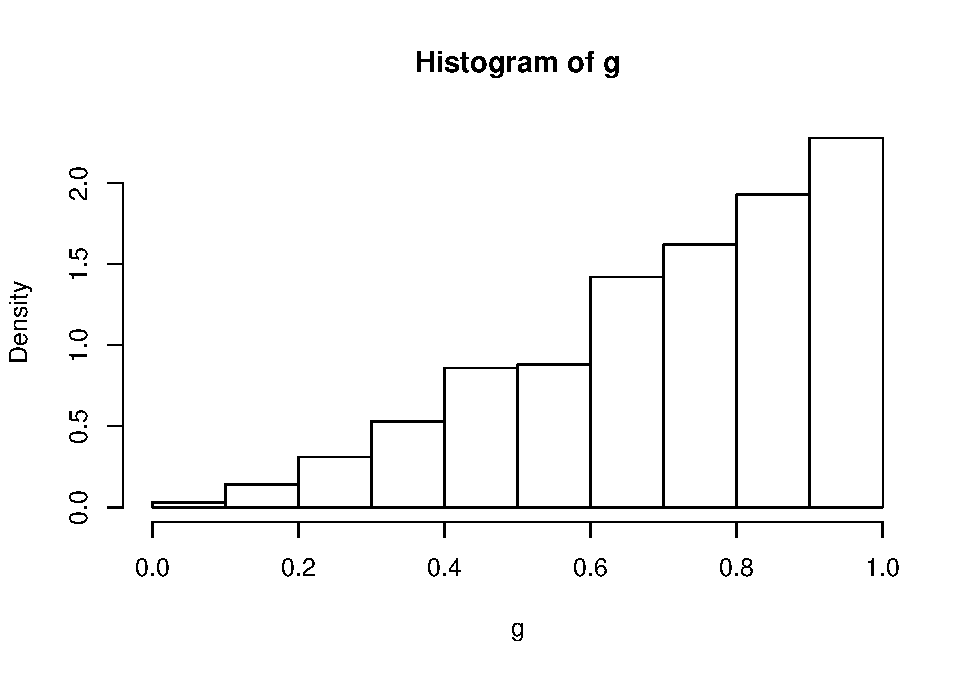
\includegraphics{hw03_yutingd3_files/figure-latex/unnamed-chunk-9-1.pdf}
\textbf{(c)} Compute the quantity
\(I_2 = \frac{1}{1000} \sum_{i=1}^{1000} \frac{f(X_i)}{g(X_i)}\) for
your sample from part (b). What is this quantity \(I_2\) as estimate of?
Compare it with \(I_1\).

\begin{Shaded}
\begin{Highlighting}[]
\NormalTok{m =}\StringTok{ }\DecValTok{10000}
\NormalTok{alpha =}\StringTok{ }\FloatTok{1.5}

\NormalTok{g =}\StringTok{ }\ControlFlowTok{function}\NormalTok{(x)\{}
\NormalTok{  g =}\StringTok{ }\KeywordTok{log}\NormalTok{(x}\OperatorTok{+}\DecValTok{1}\NormalTok{)}

\NormalTok{\}}

\NormalTok{u =}\StringTok{ }\KeywordTok{runif}\NormalTok{(m)}
\NormalTok{x =}\StringTok{ }\NormalTok{u}\OperatorTok{^}\NormalTok{(}\DecValTok{1}\OperatorTok{/}\NormalTok{(alpha}\OperatorTok{+}\DecValTok{1}\NormalTok{))}
\NormalTok{gfphi =}\StringTok{ }\KeywordTok{g}\NormalTok{(x)}\OperatorTok{/}\NormalTok{(}\FloatTok{2.5}\OperatorTok{*}\NormalTok{x}\OperatorTok{^}\FloatTok{1.5}\NormalTok{)}
\NormalTok{I2 =}\StringTok{ }\KeywordTok{mean}\NormalTok{(gfphi)}
\NormalTok{I2}
\end{Highlighting}
\end{Shaded}

\begin{verbatim}
## [1] 0.3861
\end{verbatim}

I2 is estimating \$ \int\_0\^{}1 f(x) ; dx\$. \textbf{(d)} Repeat steps
(b) and (c) 1000 times and find the standard error of the estimator I2.
Compare this error with the error E0 from Exercise 3(b).

\begin{Shaded}
\begin{Highlighting}[]
\NormalTok{m =}\StringTok{ }\DecValTok{10000}
\NormalTok{alpha =}\StringTok{ }\FloatTok{1.5}

\NormalTok{fg =}\StringTok{ }\ControlFlowTok{function}\NormalTok{(x)\{}
\NormalTok{  f =}\StringTok{ }\KeywordTok{log}\NormalTok{(x}\OperatorTok{+}\DecValTok{1}\NormalTok{)}
\NormalTok{  g =}\StringTok{ }\NormalTok{(x}\OperatorTok{>}\DecValTok{0}\NormalTok{)}\OperatorTok{*}\NormalTok{(x}\OperatorTok{<}\DecValTok{1}\NormalTok{)}
\NormalTok{  f}\OperatorTok{*}\NormalTok{g}
\NormalTok{\}}


\NormalTok{estimates =}\StringTok{ }\KeywordTok{numeric}\NormalTok{()}

\ControlFlowTok{for}\NormalTok{(i }\ControlFlowTok{in} \DecValTok{1}\OperatorTok{:}\NormalTok{m)\{}
\NormalTok{  x =}\StringTok{ }\KeywordTok{runif}\NormalTok{(}\DecValTok{1000}\NormalTok{)}\OperatorTok{^}\NormalTok{(}\DecValTok{1}\OperatorTok{/}\NormalTok{(alpha}\OperatorTok{+}\DecValTok{1}\NormalTok{))}
\NormalTok{  gfphi =}\StringTok{ }\KeywordTok{g}\NormalTok{(x)}\OperatorTok{/}\NormalTok{((}\DecValTok{1}\OperatorTok{+}\NormalTok{alpha)}\OperatorTok{*}\NormalTok{x}\OperatorTok{^}\NormalTok{alpha)}
\NormalTok{  estimates[i] =}\StringTok{ }\KeywordTok{mean}\NormalTok{(gfphi)}
\NormalTok{\}}

\NormalTok{E2 =}\StringTok{ }\KeywordTok{sd}\NormalTok{(estimates)}
\NormalTok{E2}
\end{Highlighting}
\end{Shaded}

\begin{verbatim}
## [1] 0.004383
\end{verbatim}

E2 is smaller.

\hypertarget{exercise-5}{%
\subsection{Exercise 5}\label{exercise-5}}

\textbf{Stratified Sampling.} Sometimes, it can be beneficial to divide
the interval into pieces (strata). Consider
\[ \int_{-3}^3 x^3(e^x-1) \; dx\].

\textbf{(a)} Graph the function over the range of interest. Is the
function fairly constant? Does it vary? What patterns do you see?

\textbf{(b)} Use standard Monte Carlo integration with \(k = 10,000\)
iterations to approximate this integral. Call this approximate value
\(S_0\).

\textbf{(c)} Split the function into six equal strata, (-3,-2), (-2,-1),
\ldots{} and (2,3). Use Monte Carlo integration to approximate the first
strata using \(k=10,000/6\), and the do the same with the other five
strata. Combine the results, and call this approximate value \(S_1\).

\textbf{(d)} Repeat steps (b) and (c) 1000 times and find the standard
error of both estimates. Which estimator is more efficient? Can you
think of better places to split the interval to get a more efficient
estimator?

Do the following problems from the book: 5.2, 5.4, 5.13, 5.14.

\hypertarget{solution-5}{%
\subsection{Solution 5}\label{solution-5}}

\textbf{(a)} Graph the function over the range of interest. Is the
function fairly constant? Does it vary? What patterns do you see?

\begin{Shaded}
\begin{Highlighting}[]
\NormalTok{f <-}\StringTok{ }\ControlFlowTok{function}\NormalTok{(x) x}\OperatorTok{^}\DecValTok{3}\OperatorTok{*}\NormalTok{(}\KeywordTok{exp}\NormalTok{(x)}\OperatorTok{-}\DecValTok{1}\NormalTok{)}
\KeywordTok{plot}\NormalTok{(f, }\DataTypeTok{from =} \DecValTok{-3}\NormalTok{, }\DataTypeTok{to =} \DecValTok{3}\NormalTok{)}
\end{Highlighting}
\end{Shaded}

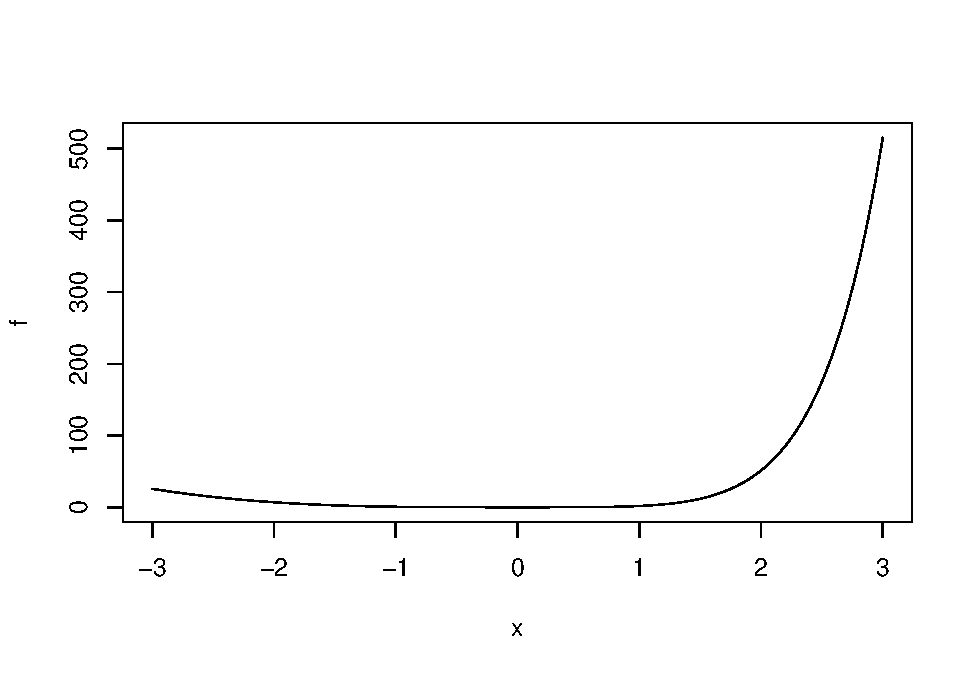
\includegraphics{hw03_yutingd3_files/figure-latex/unnamed-chunk-12-1.pdf}
\textbf{(b)} Use standard Monte Carlo integration with \(k = 10,000\)
iterations to approximate this integral. Call this approximate value
\(S_0\).

\begin{Shaded}
\begin{Highlighting}[]
\NormalTok{u <-}\StringTok{ }\KeywordTok{runif}\NormalTok{(}\DecValTok{10000}\NormalTok{, }\DecValTok{-3}\NormalTok{, }\DecValTok{3}\NormalTok{)}
\NormalTok{s0 <-}\StringTok{ }\DecValTok{6}\OperatorTok{*}\KeywordTok{mean}\NormalTok{(u}\OperatorTok{^}\DecValTok{3}\OperatorTok{*}\NormalTok{(}\KeywordTok{exp}\NormalTok{(u)}\OperatorTok{-}\DecValTok{1}\NormalTok{))}
\NormalTok{s0}
\end{Highlighting}
\end{Shaded}

\begin{verbatim}
## [1] 250.3
\end{verbatim}

\textbf{(c)} Split the function into six equal strata, (-3,-2), (-2,-1),
\ldots{} and (2,3). Use Monte Carlo integration to approximate the first
strata using \(k=10,000/6\), and the do the same with the other five
strata. Combine the results, and call this approximate value \(S_1\).

\begin{verbatim}
## [1] 222.3
\end{verbatim}

\textbf{(d)} Repeat steps (b) and (c) 1000 times and find the standard
error of both estimates. Which estimator is more efficient? Can you
think of better places to split the interval to get a more efficient
estimator?

\begin{Shaded}
\begin{Highlighting}[]
\NormalTok{n <-}\StringTok{ }\DecValTok{1000}
\NormalTok{estimates <-}\StringTok{ }\KeywordTok{matrix}\NormalTok{(}\DecValTok{0}\NormalTok{, n, }\DecValTok{2}\NormalTok{)}

\NormalTok{m =}\StringTok{ }\DecValTok{10000}
\NormalTok{k =}\StringTok{ }\DecValTok{6}
\NormalTok{S1 =}\StringTok{ }\KeywordTok{numeric}\NormalTok{(k)}

\NormalTok{g =}\StringTok{ }\ControlFlowTok{function}\NormalTok{(x)\{}
\NormalTok{  x}\OperatorTok{^}\DecValTok{3}\OperatorTok{*}\NormalTok{(}\KeywordTok{exp}\NormalTok{(x)}\OperatorTok{-}\DecValTok{1}\NormalTok{)}
\NormalTok{\}}

\ControlFlowTok{for}\NormalTok{(i }\ControlFlowTok{in} \DecValTok{1}\OperatorTok{:}\NormalTok{n)\{}
\NormalTok{  estimates[i, }\DecValTok{1}\NormalTok{] =}\StringTok{ }\DecValTok{6}\OperatorTok{*}\KeywordTok{mean}\NormalTok{(}\KeywordTok{g}\NormalTok{(}\KeywordTok{runif}\NormalTok{(m, }\DecValTok{-3}\NormalTok{, }\DecValTok{3}\NormalTok{)))}
  
  \ControlFlowTok{for}\NormalTok{(j }\ControlFlowTok{in} \DecValTok{-3}\OperatorTok{:}\DecValTok{3}\NormalTok{)\{}
\NormalTok{  S1[j] =}\StringTok{ }\KeywordTok{mean}\NormalTok{(}\KeywordTok{g}\NormalTok{(}\KeywordTok{runif}\NormalTok{(m}\OperatorTok{/}\NormalTok{k, j}\DecValTok{-1}\NormalTok{, j)))}
\NormalTok{  \}}
  
\NormalTok{  estimates[i, }\DecValTok{2}\NormalTok{] =}\StringTok{ }\KeywordTok{sum}\NormalTok{(S1)}
\NormalTok{\}}


\KeywordTok{apply}\NormalTok{(estimates, }\DecValTok{2}\NormalTok{, mean)}
\end{Highlighting}
\end{Shaded}

\begin{verbatim}
## [1] 245.0 235.6
\end{verbatim}

\begin{Shaded}
\begin{Highlighting}[]
\KeywordTok{apply}\NormalTok{(estimates, }\DecValTok{2}\NormalTok{, var)}
\end{Highlighting}
\end{Shaded}

\begin{verbatim}
## [1] 31.23 10.59
\end{verbatim}

The second method has a smaller variance indicating it is better. Trying
to split the interval into smaller pieces may achieve a more efficient
estimator.

\hypertarget{exercise-6-5.2}{%
\subsection{Exercise 6 (5.2)}\label{exercise-6-5.2}}

Refer to Example 5.3. Compute a Monte Carlo estimate of the standard
normal cdf, by generating from the Uniform(0,x) distribution. Compare
your estimates with the normal cdf function pnorm. Compute an estimate
of the variance of your Monte Carlo estimate of \(\Phi(2)\), and a 95\%
confidence interval for \(\Phi(2)\).

\hypertarget{solution-6}{%
\subsection{Solution 6}\label{solution-6}}

\begin{Shaded}
\begin{Highlighting}[]
\CommentTok{#refer to example 3.5}
\NormalTok{x =}\StringTok{ }\KeywordTok{seq}\NormalTok{(}\FloatTok{0.1}\NormalTok{, }\FloatTok{2.5}\NormalTok{, }\DataTypeTok{by =} \FloatTok{0.1}\NormalTok{)}
\NormalTok{u =}\StringTok{ }\KeywordTok{runif}\NormalTok{(}\DecValTok{10000}\NormalTok{)}

\NormalTok{cdf =}\StringTok{ }\KeywordTok{numeric}\NormalTok{()}
\NormalTok{se =}\StringTok{ }\KeywordTok{numeric}\NormalTok{()}

\ControlFlowTok{for}\NormalTok{ (i }\ControlFlowTok{in} \DecValTok{1}\OperatorTok{:}\KeywordTok{length}\NormalTok{(x)) \{}
\NormalTok{  u =}\StringTok{ }\KeywordTok{runif}\NormalTok{(}\DecValTok{10000}\NormalTok{, }\DecValTok{0}\NormalTok{, x[i])}
\NormalTok{  gx =}\StringTok{ }\KeywordTok{exp}\NormalTok{(}\OperatorTok{-}\NormalTok{u}\OperatorTok{^}\DecValTok{2} \OperatorTok{/}\StringTok{ }\DecValTok{2}\NormalTok{)}
\NormalTok{  cdf[i] =}\StringTok{ }\NormalTok{x[i]}\OperatorTok{*}\KeywordTok{mean}\NormalTok{(gx)}\OperatorTok{/}\KeywordTok{sqrt}\NormalTok{(}\DecValTok{2}\OperatorTok{*}\NormalTok{pi) }\OperatorTok{+}\StringTok{ }\FloatTok{0.5}
\NormalTok{  se[i] =}\StringTok{ }\NormalTok{x[i]}\OperatorTok{*}\KeywordTok{sd}\NormalTok{(gx)}\OperatorTok{/}\KeywordTok{sqrt}\NormalTok{(}\DecValTok{2}\OperatorTok{*}\NormalTok{pi)}\OperatorTok{/}\KeywordTok{sqrt}\NormalTok{(}\DecValTok{10000}\NormalTok{)}
\NormalTok{\}}

\CommentTok{#cbind(x, cdf,   phi=pnorm(q = x),se)}

\KeywordTok{cbind}\NormalTok{(x, cdf,   }\DataTypeTok{phi=}\KeywordTok{pnorm}\NormalTok{(}\DataTypeTok{q =}\NormalTok{ x),se)[}\DecValTok{20}\NormalTok{,}\DecValTok{4}\NormalTok{]}\OperatorTok{^}\DecValTok{2} \CommentTok{# variance for MC estimate of phi(2).}
\end{Highlighting}
\end{Shaded}

\begin{verbatim}
##        se 
## 5.303e-06
\end{verbatim}

\begin{Shaded}
\begin{Highlighting}[]
\KeywordTok{cbind}\NormalTok{(x, cdf, }\DataTypeTok{phi=}\KeywordTok{pnorm}\NormalTok{(}\DataTypeTok{q =}\NormalTok{ x),se)[}\DecValTok{20}\NormalTok{,}\DecValTok{2}\NormalTok{]}\OperatorTok{+}\KeywordTok{cbind}\NormalTok{(x, cdf, }\DataTypeTok{phi=}\KeywordTok{pnorm}\NormalTok{(}\DataTypeTok{q =}\NormalTok{ x),se)[}\DecValTok{20}\NormalTok{,}\DecValTok{4}\NormalTok{]}\OperatorTok{*}\KeywordTok{c}\NormalTok{(}\OperatorTok{-}\FloatTok{1.96}\NormalTok{,}\FloatTok{1.96}\NormalTok{) }\CommentTok{# 95% CI for MC estimate of phi(2).}
\end{Highlighting}
\end{Shaded}

\begin{verbatim}
## [1] 0.9735 0.9825
\end{verbatim}

\hypertarget{exercise-7-5.4}{%
\subsection{Exercise 7 (5.4)}\label{exercise-7-5.4}}

Write a function to compute a Monte Carlo estimate of the Beta(3, 3)
cdf, and use the function to estimate F (x) for
\(x = 0.1,0.2,\ldots 0.9\). Compare the estimates with the values
returned by the pbeta function in R.

\hypertarget{solution-7}{%
\subsection{Solution 7}\label{solution-7}}

\begin{Shaded}
\begin{Highlighting}[]
\NormalTok{f <-}\StringTok{ }\ControlFlowTok{function}\NormalTok{(x)\{}
\NormalTok{  x}\OperatorTok{^}\DecValTok{2} \OperatorTok{*}\StringTok{ }\NormalTok{(}\DecValTok{1}\OperatorTok{-}\NormalTok{x)}\OperatorTok{^}\DecValTok{2}
\NormalTok{\}}

\NormalTok{beta <-}\StringTok{ }\ControlFlowTok{function}\NormalTok{(x)\{}
  \ControlFlowTok{if}\NormalTok{(x }\OperatorTok{<=}\StringTok{ }\DecValTok{0}\NormalTok{) \{}\KeywordTok{return}\NormalTok{ (}\DecValTok{0}\NormalTok{)\}}
  \ControlFlowTok{if}\NormalTok{(x }\OperatorTok{>=}\StringTok{ }\DecValTok{1}\NormalTok{) \{}\KeywordTok{return}\NormalTok{ (}\DecValTok{1}\NormalTok{)\}}
  
\NormalTok{  c <-}\StringTok{ }\DecValTok{1}\OperatorTok{/}\KeywordTok{integrate}\NormalTok{(f, }\DecValTok{0}\NormalTok{, }\DecValTok{1}\NormalTok{)}\OperatorTok{$}\NormalTok{val}
\NormalTok{  u <-}\StringTok{ }\KeywordTok{runif}\NormalTok{(}\DecValTok{2000}\NormalTok{, }\DecValTok{0}\NormalTok{, x)}
\NormalTok{  ret <-}\StringTok{ }\NormalTok{x}\OperatorTok{*}\NormalTok{c}\OperatorTok{*}\KeywordTok{mean}\NormalTok{(}\KeywordTok{f}\NormalTok{(u))}
  \KeywordTok{return}\NormalTok{ (ret)}
\NormalTok{\}}

\NormalTok{x <-}\StringTok{ }\KeywordTok{seq}\NormalTok{(}\FloatTok{0.1}\NormalTok{, }\FloatTok{0.9}\NormalTok{, }\FloatTok{0.1}\NormalTok{)}
\NormalTok{cdf <-}\StringTok{ }\KeywordTok{numeric}\NormalTok{()}

\ControlFlowTok{for}\NormalTok{( i }\ControlFlowTok{in} \DecValTok{1}\OperatorTok{:}\DecValTok{9}\NormalTok{) \{}
\NormalTok{  cdf[i] <-}\StringTok{ }\KeywordTok{beta}\NormalTok{(x[i])}
\NormalTok{\}}

\NormalTok{true_cdf <-}\StringTok{ }\KeywordTok{pbeta}\NormalTok{(x, }\DecValTok{3}\NormalTok{, }\DecValTok{3}\NormalTok{)}

\KeywordTok{data.frame}\NormalTok{(x, cdf, true_cdf, }\KeywordTok{abs}\NormalTok{(true_cdf }\OperatorTok{-}\StringTok{ }\NormalTok{cdf))}
\end{Highlighting}
\end{Shaded}

\begin{verbatim}
##     x      cdf true_cdf abs.true_cdf...cdf.
## 1 0.1 0.008308  0.00856           0.0002517
## 2 0.2 0.058873  0.05792           0.0009527
## 3 0.3 0.164424  0.16308           0.0013438
## 4 0.4 0.320383  0.31744           0.0029434
## 5 0.5 0.522018  0.50000           0.0220176
## 6 0.6 0.665760  0.68256           0.0168003
## 7 0.7 0.834583  0.83692           0.0023374
## 8 0.8 0.938652  0.94208           0.0034285
## 9 0.9 0.994620  0.99144           0.0031796
\end{verbatim}

\begin{Shaded}
\begin{Highlighting}[]
\CommentTok{#similar result}
\end{Highlighting}
\end{Shaded}

\hypertarget{exercise-8-5.13}{%
\subsection{Exercise 8 (5.13)}\label{exercise-8-5.13}}

Find two importance functions f1 and f2 that are supported on
\((1,\infty)\) and are `close' to
\[g(x) = \frac{x^2}{\sqrt{2\pi}} e^{-\frac{x^2}{2}} \quad x>1\]

Which of your two importance functions should produce the smaller
variance in estimating
\[\int_1^{\infty}\frac{x^2}{\sqrt{2\pi}} e^{-\frac{x^2}{2}} dx \] by
importance sampling? Explain.

\hypertarget{solution-8}{%
\subsection{Solution 8}\label{solution-8}}

My choice for the importance fucntion is \(f_1(x) = e^{-x} \quad x>1\)
and \(f_2(x) = {x^2}\quad x>1\). Since those two importance functions
have the similar structure as the target function.

\begin{Shaded}
\begin{Highlighting}[]
\NormalTok{m =}\StringTok{ }\DecValTok{1000}
\NormalTok{theta.hat =}\StringTok{ }\KeywordTok{numeric}\NormalTok{()}
\NormalTok{se =}\StringTok{ }\KeywordTok{numeric}\NormalTok{()}

\NormalTok{gf =}\StringTok{ }\ControlFlowTok{function}\NormalTok{(x)\{}
\NormalTok{  g =}\StringTok{ }\KeywordTok{exp}\NormalTok{(}\OperatorTok{-}\NormalTok{x}\OperatorTok{^}\DecValTok{2}\OperatorTok{/}\DecValTok{2}\NormalTok{)}\OperatorTok{/}\NormalTok{(x}\OperatorTok{^}\DecValTok{2}\OperatorTok{/}\KeywordTok{sqrt}\NormalTok{(}\DecValTok{2}\OperatorTok{*}\NormalTok{pi))}
\NormalTok{  f =}\StringTok{ }\NormalTok{(x}\OperatorTok{>}\DecValTok{1}\NormalTok{)}
\NormalTok{  g}\OperatorTok{*}\NormalTok{f}
\NormalTok{\}}

\CommentTok{##try f1}
\NormalTok{x =}\StringTok{ }\KeywordTok{rexp}\NormalTok{(m, }\DecValTok{1}\NormalTok{)}
\NormalTok{gfphi =}\StringTok{ }\KeywordTok{gf}\NormalTok{(x)}\OperatorTok{/}\KeywordTok{exp}\NormalTok{(}\OperatorTok{-}\NormalTok{x)}
\NormalTok{theta.hat[}\DecValTok{1}\NormalTok{] =}\StringTok{ }\KeywordTok{mean}\NormalTok{(gfphi)}
\NormalTok{se[}\DecValTok{1}\NormalTok{] =}\StringTok{ }\KeywordTok{sd}\NormalTok{(gfphi)}\OperatorTok{/}\KeywordTok{sqrt}\NormalTok{(m)}

\CommentTok{##try f2}
\CommentTok{#use inverse cdf to similarte the f2}
\NormalTok{u =}\StringTok{ }\KeywordTok{runif}\NormalTok{(m)}
\NormalTok{x =}\StringTok{ }\NormalTok{(}\DecValTok{3}\OperatorTok{*}\NormalTok{u)}\OperatorTok{^}\NormalTok{(}\DecValTok{1}\OperatorTok{/}\DecValTok{3}\NormalTok{)}
\NormalTok{gfphi =}\StringTok{ }\KeywordTok{gf}\NormalTok{(x)}\OperatorTok{/}\NormalTok{(x}\OperatorTok{^}\DecValTok{2}\NormalTok{)}
\NormalTok{theta.hat[}\DecValTok{2}\NormalTok{] =}\StringTok{ }\KeywordTok{mean}\NormalTok{(gfphi)}
\NormalTok{se[}\DecValTok{2}\NormalTok{] =}\StringTok{ }\KeywordTok{sd}\NormalTok{(gfphi)}\OperatorTok{/}\KeywordTok{sqrt}\NormalTok{(m)}


\NormalTok{se}
\end{Highlighting}
\end{Shaded}

\begin{verbatim}
## [1] 0.03189 0.01221
\end{verbatim}

It seems like \(f_2(x) = {x^2}\quad x>1\) has smaller variance which
indicating it is closer to the target function.

\hypertarget{exercise-9-5.14}{%
\subsection{Exercise 9 (5.14)}\label{exercise-9-5.14}}

Obtain a Monte Carlo estimate of
\[\int_1^{\infty}\frac{x^2}{\sqrt{2\pi}} e^{-\frac{x^2}{2}} dx \] by
importance sampling.

\hypertarget{solution-9}{%
\subsection{Solution 9}\label{solution-9}}

We can change our variable by y = 1/x, then
\[\int_1^{\infty}\frac{x^2}{\sqrt{2\pi}} e^{-\frac{x^2}{2}} dx \] will
be \[\int_0^{1}\frac{1}{y^4\sqrt{2\pi}} e^{-\frac{-1}{2y^2}} dy \]

\begin{Shaded}
\begin{Highlighting}[]
\NormalTok{n <-}\StringTok{ }\DecValTok{1000}
\NormalTok{gf <-}\StringTok{ }\ControlFlowTok{function}\NormalTok{(x)\{}
  \ControlFlowTok{if}\NormalTok{(x }\OperatorTok{<}\StringTok{ }\DecValTok{0}\NormalTok{) \{}\KeywordTok{return}\NormalTok{ (}\DecValTok{0}\NormalTok{)\}}
  \ControlFlowTok{else} \ControlFlowTok{if}\NormalTok{ (x}\OperatorTok{>}\DecValTok{1}\NormalTok{) \{}\KeywordTok{return}\NormalTok{ (}\DecValTok{0}\NormalTok{)\}}
\NormalTok{  gf =}\StringTok{ }\KeywordTok{exp}\NormalTok{(}\OperatorTok{-}\DecValTok{1}\OperatorTok{/}\NormalTok{(}\DecValTok{2}\OperatorTok{*}\NormalTok{x}\OperatorTok{^}\DecValTok{2}\NormalTok{)) }\OperatorTok{/}\StringTok{ }\NormalTok{(}\KeywordTok{sqrt}\NormalTok{(}\DecValTok{2}\OperatorTok{*}\NormalTok{pi)}\OperatorTok{*}\NormalTok{x}\OperatorTok{^}\DecValTok{4}\NormalTok{)}
  \KeywordTok{return}\NormalTok{ (gf)}
\NormalTok{\}}

\NormalTok{iter <-}\StringTok{ }\DecValTok{0}
\NormalTok{x <-}\StringTok{ }\KeywordTok{numeric}\NormalTok{()}

\ControlFlowTok{while}\NormalTok{(iter }\OperatorTok{<}\StringTok{ }\NormalTok{n)\{}
\NormalTok{  f1 <-}\StringTok{ }\KeywordTok{rexp}\NormalTok{(}\DecValTok{1}\NormalTok{)}
\NormalTok{  x[iter] <-}\StringTok{ }\KeywordTok{gf}\NormalTok{(f1)}
\NormalTok{  iter <-}\StringTok{ }\NormalTok{iter }\OperatorTok{+}\StringTok{ }\DecValTok{1}
\NormalTok{\}}

\NormalTok{gfphi =}\StringTok{ }\NormalTok{x}\OperatorTok{/}\KeywordTok{exp}\NormalTok{(}\OperatorTok{-}\NormalTok{x)}
\NormalTok{thetheta =}\StringTok{ }\KeywordTok{mean}\NormalTok{(gfphi)}
\NormalTok{thetheta}
\end{Highlighting}
\end{Shaded}

\begin{verbatim}
## [1] 0.4578
\end{verbatim}

\end{document}
